%\documentclass[11pt,a4paper,runningheads]{llncs}
\documentclass[11pt,a4paper]{article}
%encoding
%--------------------------------------
\usepackage[T1]{fontenc}
\usepackage[utf8]{inputenc}
%--------------------------------------

%Portuguese-specific commands
%--------------------------------------
\usepackage[portuguese]{babel}
%--------------------------------------

%Hyphenation rules
%--------------------------------------
\usepackage{hyphenat}
\hyphenation{mate-mática recu-perar}
%--------------------------------------

\usepackage{graphicx}
\usepackage{comment}
\usepackage{pgfplots}
\usepackage{amsmath,amssymb,amsfonts}
\usepackage{algorithmic}
\usepackage{graphicx}
\usepackage{textcomp}
\usepackage{xcolor}
\usepackage{adjustbox}
\usepackage{float}


\begin{document}

\title{Fase 3 - Requisitos, Casos de Uso e Arquitetura}
\author{Pedro Carrega, nº49480 \and
Vasco Ferreira, nº49470 \and Ye Yang, nº 49521
}

%\institute{Departamento de Informática da Faculdade de Ciências da Universidade de Lisboa
%\email{\{fc49480,fc49470,fc49521\}@alunos.fc.ul.pt}}

\maketitle

\section{Requisitos}

\begin{table}[H]
	\begin{center}
		\begin{tabular}{|p{3.5cm}|p{9.5cm}|}
		\hline
			\textbf{Requisitos\newline Não Funcionais} & \textbf{Descrição}\\ \hline
			Portabilidade & Implementação de servidor em NodeJS e cliente em JAVA de modo a facilitar o processo de mudança de plataforma do serviço \\ \hline
			Legibilidade & A separação clara entre as camadas de apresentação, lógica de negócio e acesso à base de dados irá tornar o fluxo do sistema mais legível para os desenvolvedores \\ \hline
			Estabilidade & A distribuição do sistema por diversas máquinas virtuais, que poderão estar distribuídas por diferentes fornecedores cloud e em diferentes Data Centers permitem obter um sistema estável \\ \hline
			Elasticidade & O sistema deverá ser capaz de se adaptar à carga de trabalho através do provisionamento e desprovisionamento dos recursos de forma autónoma. Idealmente, de forma que em qualquer ponto do tempo, o sistema apenas utilize o número de máquinas necessárias de forma a corresponder à carga atual \\ \hline
			Escalabilidade & Capacidade do sistema lidar com o crescimento de carga de trabalho. Pode-se associar à capacidade de elasticidade do sistema \\ \hline
			Confiabilidade & Visto o sistema estar implementado na núvem, conseguimos garantir alta confiabilidade nos sistema, pois se um servidor no datacenter falhar, conseguimos facilmente migrar a VM para outro servidor funcional \\ \hline
	\end{tabular}
	\label{tab1}
	\end{center}
	\caption{Requisitos Não Funcionais}
\end{table}

\begin{table}[H]
	\begin{center}
		\begin{tabular}{|p{3.8cm}|p{8.2cm}|}
		\hline
			\textbf{Requisitos\newline Funcionais} & \textbf{Descrição}\\ \hline
			Listar\newline Categorias Disponíveis & Serviço que fornece aos clientes todas as categorias \\ \hline
			Visualizar\newline Popularidade das\newline Marcas & Serviço que fornece cada marca associada com a sua popularidade\\ \hline
			Visualizar\newline Número de Vendas\newline Individuais & Fornece o numero total de vendas de cada marca\\ \hline
			Visualizar\newline Preço Médio de Venda & Fornece o preço médio dos produtos vendidos de uma determinada marca \\ \hline
			Visualizar\newline Rácio de Tipo\newline de Eventos & Fornece a percentagem de cada tipo de evento \\ \hline
	\end{tabular}
	\label{tab2}
	\end{center}
	\caption{Requisitos Funcionais}
\end{table}
\paragraph{}

\section{Diagrama de Casos de Uso}
\begin{figure}[H]
  \centering
  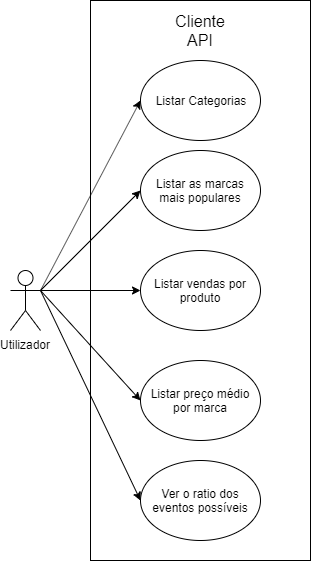
\includegraphics[scale=0.42]{Use_Cases.png}
  \caption{Diagrama de casos de uso}
\end{figure}

\section{Arquitetura da aplicação}
\begin{figure}[H]
  \centering
  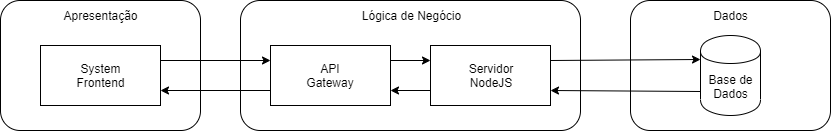
\includegraphics[scale=0.4]{App_arc.png}
  \caption{Arquitetura da aplicação}
\end{figure}

Após a definição da API com o Swagger na fase anterior, possibilitou a opção de exportar do API definido um Cliente (em Java) e um Servidor NodeJS.

\subsection{System Frontend}
O frontend irá dispor as funcionalidades anteriormente definidas. Pode ser extraído do ficheiro Swagger em formato HTML.
\newline

\subsection{API Gateway}
Este gateway irá ser encarregado de receber pedidos HTTP vindos do frontend e reencaminhá-los para o servidor NodeJS que tratará da lógica de negócio. Também irá encaminhar as respostas vindas do servidor para o frontend de modo disponibilizar os dados pretendidos.
\newline %removam isto se nao gostarem do espaço k adiciona


\subsection{Servidor NodeJS}
O servidor exportado do Swagger irá receber os pedidos a partir da API Gateway, e processá-los de acordo com a funcionalidade pretendida. A lógica de negócio é aqui tratada, realizando as queries necessárias para a base de dados. Ao receber os dados, processa-os de acordo com a funcionalidade, e encaminha o resultado para a gateway.
\newline %removam isto se nao gostarem do espaço k adiciona

\subsection{Base de dados}
A base de dados irá conter o conteúdo dos ficheiros .csv do nosso data set, que são acedidos pelo servidor de modo a poder efetuar as leituras necessárias para produzir uma resposta para o cliente. 

\section{Arquitetura técnica}
%Digam-me o que acham

%Não sei o que dizer da Portabilidade
Para garantir os requisitos não funcionais mencionados a cima devemos ter em atenção os serviços da cloud escolhidos, pois estão relacionados com os requisitos.
\newline
O facto de ser usada a cloud acaba por conseguir garantir alguns dos requisitos, como por exemplo a Elasticidade, devido ao facto de a cloud nos permitir expandir ou reduzir a capacidade do sistema. A mesma lógica se pode aplicar de forma a garantir a Escalabilidade de sistema. A capacidade de expansão referida anteriormente permite numa outra perspetiva garantir a Confiabilidade, já que permite uma fácil migração de uma máquina virtual em falha para uma outra máquina virtual funcional. 
\newline
Já a Estabilidade é garantida devido a ter a Lógica de negócio distribuída por várias máquinas virtuais que cumprem a função de servidores.

\end{document}